\chapter{A Simulation-based Exploration of Capacity}
\label{chap:capacity}
In the previous chapter, we presented a simple model for energy capacity and explored the effect of capacity on the amount of energy captured by a system. 
We utilized synthesized energy harvesting traces from an existing irradiance trace dataset, however we simplified the analysis by assuming a static average workload power.
This chapter will explore expanding our model to utilize several different dynamic workloads based off of benchmarks of real hardware, as well as considering a wireless sensor state machine that better captures the behavior of a real sensor.
The rest of the chapter is an analysis of the performance of these simulated wireless sensor workloads under real harvesting conditions.

\section{Upgrading Our Model}
\label{sec:capacity:modelling}
%The model and analysis we presented in \cref{sec:intuition:capacity} does not consider
%workload variability, and simplifies workload to an average.
In \cref{sec:intuition:capacity}, we argued that a sensor workload, which is often periodic or event driven, does not vary significantly beyond a few hours to a day of operation when compared to the variability of energy harvesting income. Photovoltaic harvesting can vary significantly over the course of a day and throughout a year. 
To verify this assumption and expand our analysis of capacity, we seek to to explore the dynamic effects that energy
capacity and backup storage have on sensor performance in the face of workload variability.
We use representative energy harvesting traces, measurements of real hardware,
and synthesized dynamic workloads in a new model based on a simple wireless sensor state machine.
We use this model to simulate
the behavior of energy harvesting sensors. 
From the input traces of workload and energy harvesting income, our model produces estimates of sensor energy utilization, availability, responsiveness, and lifetime.

\placefigure{tab:capacity:rep}

\subsection{Energy Harvesting Income}
As in \cref{sec:intuition:capacity}, we utilize the EnHANTs irradiance trace dataset as energy income for our simulation.
Unlike our previous analysis, we do not use synthesized traces, and instead utilize the traces directly.
We choose to narrow our focus to two of the traces that we think most accurately represent indoor lighting conditions: Setup A and Setup D.
As shown in \cref{fig:intuition:traces}, Setup A represents a location that receives some sunlight but is mostly lit by artificial sources while Setup D represents a location near a window that receives significant light during part of the year.
Beyond \cref{fig:intuition:traces}, these traces are summarized in \cref{tab:capacity:rep}.
On average, Setup A provides an average of 15.1\ssi[per-mode=symbol]{\micro\watt\per\centi\meter\squared} which is on the lower end of expected irradiance in indoor environments. Setup D represents the higher end of indoor irradiance with an average 97.4\ssi[per-mode=symbol]{\micro\watt\per\centi\meter\squared}.

\placefigure{tab:capacity:components}

\subsection{Representative Hardware}
We limit our analysis to the effects of capacity,
independent of the differences of energy intensity or efficiency in device
component selection. To do so, we define an example photovoltaic energy harvesting
sensor platform that utilizes currently available commercial
components. These components are listed in \cref{tab:capacity:components}.
We choose new
components in an attempt to better represent prior energy storage designs and
give them the benefit of the improvements that have occurred in recent years.
We take benchmark
measurements of various tasks performed by this representative platform, such as the
amount of time and energy required to sample a sensor or send a Bluetooth Low
Energy (BLE) packet. 
These benchmarks are used to generate energy utilization metrics
for our representative workloads shown in \cref{tab:capacity:rep}.
The physical size of the solar panel used by this sensor
is assumed to be
10.9~cm\textsuperscript{2} and the volume of the sensor node is similar to prior
work like the Hamilton sensor~\cite{kim2018system}.
%We implement this design and describe it further in \cref{sec:impl:permamote}.

\subsection{Representative Workloads}
We find that sensing workloads generally fall into three
categories: (i) periodic sense-and-send~\cite{mainwaring2002wireless}, (ii) reactive event detection~\cite{campbellEnergy14,afanasov2020battery}, and (iii) infrequent,
long-running, high-energy events~\cite{levis2004trickle}. 
All of these workloads are characterized by long periods in which a sensor is inactive, punctuated by active events, which may be periodic or drawn from a distribution.
These active events may correspond to collecting a measurement from a sensor, performing some computation, and transmitting the results.
We choose a representative workload for each
of the three categories to use in our model.
We characterize our ``periodic sense-and-send''
workload as periodically sampling a light and three channel color sensor and sending a
BLE advertisement containing the data.
Our ``reactive workload'' consists of sending a BLE advertisement upon motion detection of the main
entrance of a university building, and we linearly scale the frequency
of these events to create synthetic traces with varying amounts of usage. 
We treat these workloads as atomic. 
When a measurement is taken or a packet is sent in response to a periodic schedule or a detected event, the energy spent on those operations must be spent instantaneously and atomically. 
This means a sensor must currently have sufficient energy stored to complete the operation, otherwise the event is considered ``missed'' and counted against the availability of the system.
Finally, our ``infrequent expensive'' workload is a
contiguous
task that is representative of an
over-the-air firmware update, which is randomly executed with an average occurrence rate
of once every two weeks.
We optimistically assume this long running task can be interrupted
and resumed at any point during execution and that any checkpointing does not incur any overhead.

\placefigure[t]{tab:parameters}

\section{An Energy Model for Wireless Sensors}
We use the previously discussed indoor irradiance traces, generalized
workloads, and hardware characterizations to model the behavior of sensors
using different types and sizes of energy storage. We develop an open
source\footnote{\url{https://github.com/lab11/permamote/tree/master/simulator}}
iterative simulator that allows parameterization of various system
characteristics, including regulator efficiency, solar harvester size
and efficiency, energy storage capacity, leakage, equivalent series resistance (ESR), and charge-discharge
efficiency. These parameters are summarized in \cref{tab:parameters}.

The simulation of our model operates as a second-by-second calculation of the
amount of energy entering and exiting a device, similar to the model presented in \cref{sec:intuition:capacity}.
At every step, the simulation calculates the net energy gain or loss of the
system based on its current state, the instantaneous harvestable energy, and available stored energy.  
Occasionally,
the model performs a workload event based on either a periodic schedule (in the
case of a sense-and-send workload) or from a random distribution (reactive
event detection or a high-energy event). For our modeling, workload schedules
are generated from values listed in \cref{tab:capacity:rep}.
This simulation is performed for the entirety of an
input irradiance trace, which constitutes about a year of data. During
a simulation, metrics such as energy utilization, the fraction of completed
events versus expected events, and event time to completion are collected,
and if applicable, the primary-cell lifetime is estimated from a trace of its capacity over time.

\placefigure{fig:capacity:statemachine}

During simulation, modeled devices can be online or offline and idle or performing
work. These states are shown in \cref{fig:capacity:statemachine}.  A device's state
transitions from top to bottom of this figure and vice versa depending on the
energy state of the secondary storage.
If the secondary-cell energy state drops below \texttt{min\_hyst},
the state of the system moves to the upper
half (\textsf{offline}) of this diagram. The state of the system moves downward (\textsf{online})
if the state of charge of the secondary reaches the \texttt{max\_hyst}
limit. 
Secondary charging hysteresis limits are defined by parameters described in \cref{tab:parameters}.
A device's state can also move
to the right or left of the state machine depending on whether a workload event
is scheduled, or the prescribed workload has been completed. A new
workload event is counted as failed if the device is not in the \textsf{Online
Idle} state when it begins.
In the case of the ``atomic''
sense-and-send and reactive workloads, the modeled device will only begin
to perform an expected workload event if it has
enough energy to perform the event in entirety. If the workload is not atomic,
the device will only begin scheduled work if it has enough energy to make the
configured minimum amount of progress. We
make an assumption that the duration of atomic events are less than the one
second simulation step.
We also assume that a modeled sensor has perfect, zero-energy progress
latching and can go to sleep at any point after an active event. 
If there is energy remaining after performing a task, the modeled sensor will
attempt to spend the rest of the simulation period in the \textsf{Online Idle} state.

If the simulated device is configured with a backup primary-cell, offline
states transform to ``primary'' states in which the device remains on and
able to perform work, but charges energy usage to the primary storage instead
of the secondary. During these periods, the secondary cell continues charging
from harvested energy. Upon reaching the upper charging hysteresis
limit, the device returns to an online state, using energy stored in the
secondary.  If the primary storage is depleted, the simulation ends early.

\placefigure{fig:usage}

\section{Capacity Increases Energy Capture and Availability}
\label{sec:capacity:capture}

Using our simulator, we can confirm that the conclusions 
from \cref{sec:intuition:capacity}
regarding the relationship between energy capacity and energy capture. 
An increase in sensor energy capacity results in an increase in the capture of energy during periods of abundant harvestable energy.
This additional energy has the effect of increasing the availability of the sensor, as the buffer serves to average out times of energy insufficiency and excess.
Higher
The next few subsections explore the effect of capacity on energy utilization and sensor availability.

\subsection{Ambient Energy Utilization}
\label{sec:capacity:utilization}

Ambient energy is underutilized when it is not used to support the specified
sensing application. This may happen for two reasons: 1) 
the secondary
energy storage is full but energy is still available for harvesting, and 2) the
sensor performs work based on its energy state rather than its application
goals. The first scenario is common for energy harvesting systems
presented in prior work that charge up a capacitor and wait for an event
before sensing and sending, failing to capture all energy that may
have been harvested while their capacitor was full~\cite{campbellEnergy14, afanasov2020battery}.
For an example of the second scenario, consider
systems that transmit a packet every time their energy storage capacitor
is full rather than saving this energy for use during periods of lower harvesting
potential~\cite{hesterFlicker17, colinReconfigurable18}. Another example of this are sensors in which the harvesting
rate is proportional to the sensed phenomena~\cite{debruin2013monjolo}.

To explore ambient energy utilization as a function of storage size, we
use our simulation of the charge-discharge patterns of idealized energy stores under
the harvesting conditions and workloads described in \cref{sec:capacity:modelling}.
We perform multiple simulation runs while sweeping energy storage capacity and measuring the amount of harvestable energy captured and used by the intended workload.
We desire to isolate the effect of capacity from the type of storage, so the
idealized energy storage is assumed to have no leakage or ESR. 
%Our simulator is capable of considering these sources of inefficiency. 
%However, leakage and ESR are more dependent on the type of energy storage than the capacity, 
%making a sweep through capacity more complex than necessary when considering them.
This modeling is primarily accounting for our first classification of
wasted energy, since our workload definitions \textit{do not} perform
tasks in response to available energy; instead they attempt to maximize the success
rates for the specified sensing tasks.
The results of this modeling are shown in \cref{fig:usage}.
No matter the amount of available energy or the workload considered, energy utilization increases as
storage capacity increases. For scenarios with low harvesting potential and high
power workloads, a sensor with at least 1\ssi{\milli\Wh} of storage can accomplish 100\% utilization.
In cases of
high harvesting potential and low power workloads, utilization often
stops increasing before reaching 100\%. This
can be attributed to a small fraction of the available energy being sufficient
to fully support the sensing task.
The x-axis of \cref{fig:usage} is split by energy capacities possible with capacitors, supercapacitors, and
batteries. 
The upper extents of capacity for capacitors represents ten 100\,\si{\micro\farad} tantalum capacitors~\cite{tantalumDatasheet}. 
For supercapacitors, the extent is represented by one
large 220\,mF supercapacitor~\cite{murataCap}. 
These delineations are not hard partitions, as capacitors and supercapacitors have a wide range of capacities and the capacities offered can overlap in some configurations.
In most cases, energy utilization is maximized with energy capacity characteristic of small batteries or large supercapacitors.
For the low light, 15\ssi[per-mode=symbol]{\micro\watt\per\centi\meter\squared}, environment, a few of the workloads are eventually able to harvest 100\% of the available light as capacity increases. This indicates that the sensor performance is bounded by available harvestable energy, which is not enough to sustain the workload.
Conversely, in the high light 97\ssi[per-mode=symbol]{\micro\watt\per\centi\meter\squared} environment, regardless of the workload, the simulated sensors are not harvesting all or even the majority of the available energy. 
This indicates they are harvesting as much as needed to power their workload. 

\placefigure{fig:capacity:availability}
\placefigure{fig:capacity:period}

\subsection{Workload Availability}
\label{sec:capacity:availability}

In addition to energy utilization we also measure the ability of varying energy stores to meet the chosen 
sensing tasks and intensities. 
The results are
shown in \cref{fig:capacity:availability}. 
Similar to the results of \cref{fig:capacity:availability}, we see marked
increases in performance when the amount of energy capacity reaches 1-10\,mWh
of capacity.
Simulations experience 100\% availability for all but
the most energy constrained scenarios with high power workloads and
$\geq$2\,mWh of energy storage.
\Cref{fig:capacity:period} is another view of availability, and examines sweeping the period of the periodic workload with four decades of energy capacity.
This figure shows that even 
with gratuitous energy harvesting potentials and infrequent workloads, sensors with low energy capacity experience low
availability.
This is because they
unable to capture enough energy to allow continuous sensing through periods with little to no harvestable energy, like nighttime or winter. 

\subsection{Workload Timeliness}
\placefigure{fig:capacity:ttc}
\placefigure{fig:primary}
Finally, we analyze the ability of different storage configurations to perform a 
long-running, contiguous, higher energy task. 
The characteristics of the long-running task are presented in \cref{tab:capacity:rep_work}. We 
This long-running task is an example of a medium-sized, 50\ssi{\kilo\byte} over-the-air code update.
\Cref{fig:capacity:ttc} is a CDF of the time-to-completion for this update with different configurations of energy capacity, workload, and harvesting conditions.
Nearly all of the configurations with
0.28\,mWh of energy storage can complete the task in the minimum amount of time (5\,s). In comparison,
even reducing the amount of energy storage to match the amount of energy
required for an update causes significant latency. 
Many of the updates for smaller energy storage configurations
do not complete for 1000-10,000\,s.
This aligns with the amount of time a sensor may sit
idle overnight waiting for power from daytime to continue and eventually complete its update.



% Mayfly/Flicker
% - Timekeeper: 1 10uF 0805YD106KAT2A 0.09 @ 100 (equiv 0.03 @ 100) (0.023)
% - MCU: 1 22uF Not specified, but an AVX 1210 costs 0.44 @ 100 (equiv 0.079 @ 100) (0.025)
% - Acel 1 2.2uF EMK107BJ225KA-T 0.039 @ 100 (equiv 0.036 @ 100) (0.015)
% - BLE  1 47uF GRM31CR60J476ME 0.21 @ 100 (equiv 0.16 @ 100) (0.028)
% - HUM  1 15uF C2012X7S1A156M125AC 0.37 @ 100 (equiv 0.19 @ 100) (0.052)
% - Press 1 33uF C3216X5R0J336M130AC 0.44 @ 100 (equiv 0.38 @ 100) (0.034)
%
% Capybara
% - test 1: 400uF ceramic (4x100 0.31 equive @100) (0.043), 330uF tant (0.69 equiv @100) (0.24), 67.5 mF super (?? $21?, $2.42)
% - test 2: 300uF ceramic (3x100), 1100uF tant ($2.43) (0.62), 7.5 mF super ($2.42) (
% - test 3: 300uF cerami (3x100)c, 100uF tant ($0.28) (0.17), 7.5 mF super ($2.42)
%
% Gecko Power Supply
% - 5 TLJG227M004R3000 1.39 @ 100 (0.37 equiv, 0.16 ali)
%
% Wisp
% - 1 10uF ?? $0.05 @ 100
\begin{definefigure}{fig:primary}
  \centering
  \begin{subfigure}{\columnwidth}
    \centering
    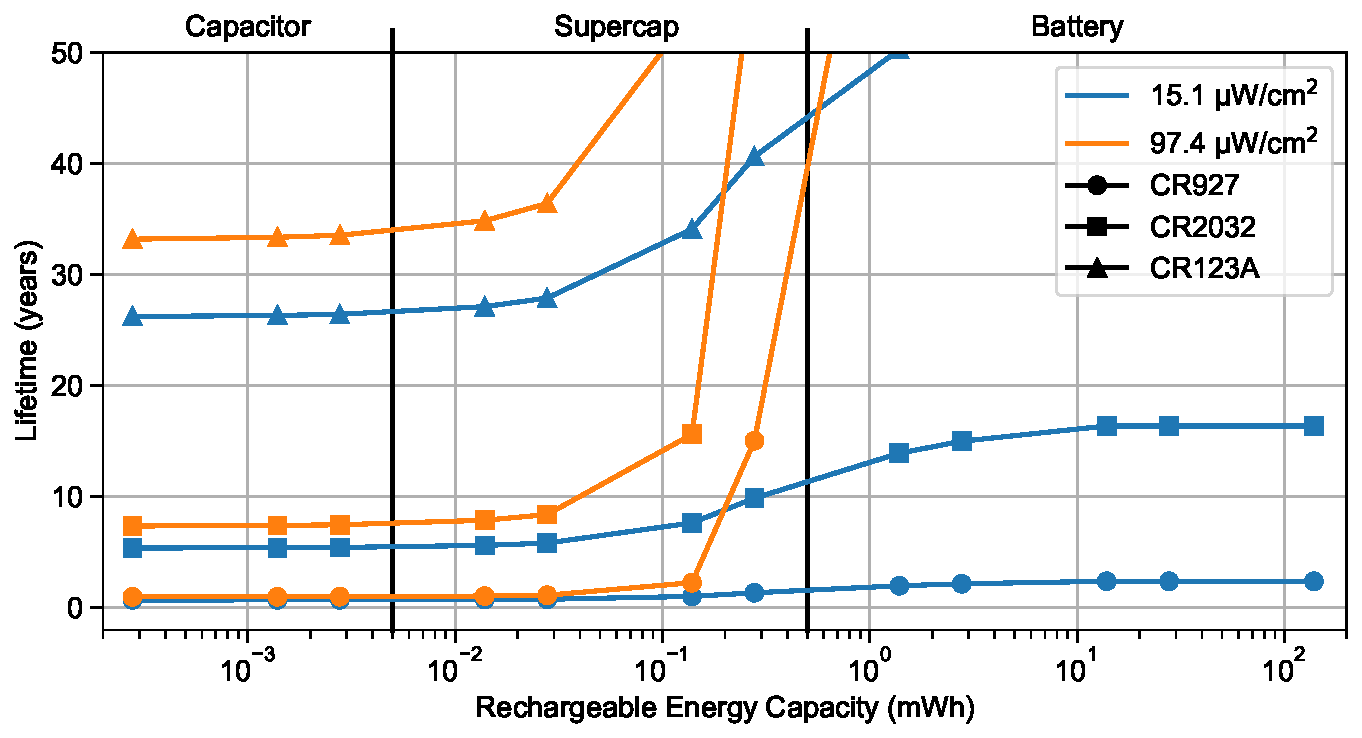
\includegraphics[width=\linewidth]{figs/capacity/primary/sense_and_send_life_vs_sec_size}
    \caption{Periodic Application}
    \label{fig:primary:sensesec}
  \end{subfigure}
  \begin{subfigure}{\columnwidth}
    \centering
    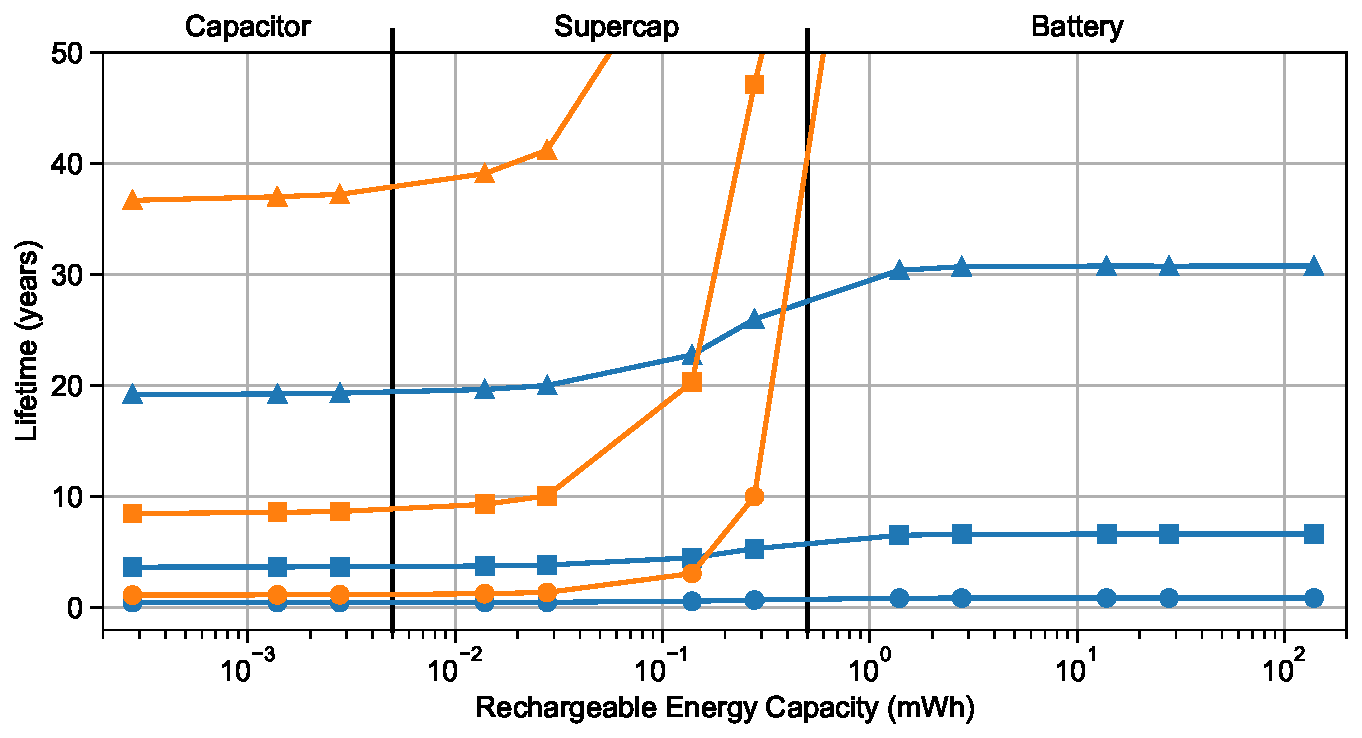
\includegraphics[width=\linewidth]{figs/capacity/primary/door_occu_life_vs_sec_size}
      \caption{Reactive Application}
    \label{fig:primary:eventsec}
  \end{subfigure}
  \caption{
    \normalfont
    Estimated lifetime
    when varying secondary energy capacity for different harvesting scenarios
    and backup energy storage sizes. 
    The periodic application's period
    is 30\,s and the reactive application events are scaled to
    represent a maximum of 2000 events per hour during the peak hour.
    %Harvesting scenarios and workloads
    %are described in \cref{sec:overview} and \cref{tab:capacity:rep}, and
    The backup
    sizes correspond to those found in common coin cell batteries:
    90\,mWh, 720\,mWh, 4500\,mWh for the CR927, CR2032, and CR123A respectively.
    As the ability to capture
    more harvested energy increases, the sensors lifetime increases.
    In some scenarios, expected
    lifetime becomes unbounded as the device is able to subsist entirely on harvested
    energy.
    %All scenarios experience substantial
    %increases in lifetime from increased secondary storage size.
    }
\end{definefigure}

\section{Availability Requires Backup}
\label{sec:primary:availability}

Increasing secondary capacity greatly improves
availability across all workloads.
%for both periodic and reactive workloads.
However, some environmental
conditions and workloads do not reach 100\% availability regardless of the size
of the secondary store.
Some workloads simply require more energy
than is available to harvest, and can not achieve high availability because they already capture all the energy they can.
%reactive workloads with large secondary
%capacities, some of the
For systems that can theoretically capture enough energy on average, they still may experience periods where they run out of stored energy.
Some of the results in \cref{fig:capacity:availability}
that appear to achieve near 100\% availability actually miss between 0.1 and 2\% of events because they did not initially start with enough energy stored.
%with
%diminishing returns for increased secondary capacity.
%Additionally, some workloads
In both of these cases, a backup energy store can increase availability 
to 100\%.
However, the introduction of a non-rechargeable backup means a system now has a finite lifetime.
%In both of these case, further increasing secondary
%capacity does not improve availability.
%and the desired application cannot rely soly on harvested power.
%and we expect that
%workloads which achieve slightly less than perfect availability are experiencing
%a combination of brief harvesting droughts and high amounts of temporally local activity
%that push the local average power well above that of the average harvested power.
While the second case may be solved with a sufficiently large secondary-cell that is deployed fully charged, the
diminishing returns of increasing secondary size and
unpredictability of some reactive applications
makes it difficult to rely solely on harvested power.

We argue that 100\% availability is a significant improvement over
even low failure rates with respect to availability
%information
%for many applications
and simplicity due to the lack of intermittency.
%that is a consequence
%of availability.
As we discuss in \cref{sec:background:app}, many types of applications 
must provide high availability to be successful.
For applications that are human facing, research suggests that any unavailability
results in frustration and %lack of
unwillingness to adopt automated solutions~\cite{brushHome11, edwardsHome01, shehanHome07}.
To use energy harvesting sensors for human-facing applications, ones that control safety-critical systems, or applications that simply require consistent and periodic sensing, inherent unavailability is intolerable.
Beyond the availability of the normal sensor workload, it is also important to be able to detect and identify the failures in a sensor deployment.
Batteryless system failures are difficult to detect %and mitigate
because there is no method for differentiating between lack of energy
and an actual fault. While scheduled communication of current energy state
may help, this would be difficult for systems that only store enough
energy to perform a single operation~\cite{hesterFlicker17, yervaGrafting12, colinReconfigurable18,campbell2018energy}.
The only way to ensure there is \textit{always} energy available to issue a heartbeat message or report issues, a backup non-rechargeable source of energy is required.

%Finally, it is more difficult
%to program intermittent systems because programmers or the underlying
%programming model must monitor and adapt to available energy with fine
%granularity, both of which are non-trivial tasks.
%These systems have little ability to correct for failures
%even when they are detected.
%A reliable system has the ability to spend more short-term
%energy to correct for detected failures.

\subsection{Lifetime of a Backup Energy Store}
\label{sec:primary:lifetime}

To achieve 100\% availability and avoid frequent power and state loss,
designs can utilize a backup energy store.
In this section we simulate the workloads of energy harvesting sensors with backup non-rechargeable energy storage.
In instances where the rechargeable source is depleted, the system
can operate from the backup, masking the effects of variable energy income.
We estimate the lifetime of the backup based on the discharge rate resulting from the simulated workload. 
We consider a sensor's lifetime to be completed when its backup energy store is depleted.
We assume the backup energy store is  
a primary battery, as they offer very low self-discharge, long shelf life, and
superior energy density.

%that is pre-charged at the start of the
%node's life.
%This pre-charged energy store could be accomplished
%by either a large secondary-cell or a primary-cell, but to avoid increasing
%volume significantly this energy store will almost certainly manifest itself
%as a non-rechargeable battery.
An analysis of the reliable lifetime of sensors configured with energy
harvesting and a backup energy store is shown in \cref{fig:primary}.
%for
%both periodic and event based workloads.
We choose several backup energy
stores with energy equivalent to those found in several types of common
primary-cells. We see that with energy harvesting and a sufficiently
large secondary energy store, nodes can
achieve 100\% reliable lifetimes that exceed
what we can reasonably predict, especially for harvesting scenarios that
exceed the average power of the application. In these scenarios, 
the inclusion of a backup energy store is critical 
to ensure availability in uncharacteristically adverse conditions.
Even for conditions with
limited energy availability we still observe significant lifetime improvements
due to energy harvesting.
We identify a 2-4x increase in lifetime estimates from the smallest to largest
capacity simulated, if we only consider bounded results.
In some cases, lifetime estimates grow exponentially as rechargeable energy capacity is increased, indicating that with sufficient capacity and income, a workload almost never needs to utilize the energy in its non-rechargeable backup.
These results confirm the initial analysis performed in \cref{sec:intuition:hybrid}, which showed substantial lifetime improvements when considering hybrid energy harvesting systems with backup preallocated energy.
We emphasize that
these lifetime estimations are
just estimations, and while we do model the 1\,\%/year leakage
typical of coin cells, we do not consider the unknown
physical or chemical degradation that would be experienced over decades of use or in adverse environments.

\section{Summary}
In this chapter, we present an upgraded energy harvesting and storage model and use it to simulate the behavior and common workloads of wireless sensors.
This simulation improves upon the simple analysis performed in \cref{sec:intuition:capacity} by considering a dynamic workload, more realistic energy income and energy storage characteristics, and the effects of preallocated backup energy storage.
We use the results from multiple simulation runs to illustrate the impact of energy capacity on the performance of wireless sensors.
Increasing energy capacity allows a system to increase its energy utilization. In turn, increased energy utilization allows a wireless sensor to more successfully complete its workload, regardless of the type or distribution of workload activity.
Despite the improvements granted by increased capacity, a wireless energy harvesting sensor will still be limited by the magnitude of available harvestable energy.
In cases where harvestable energy is insufficient to power an intended application workload, it can be beneficial to include a backup non-rechargeable source of energy to ensure high availability.
While this inclusion results in a wireless sensor with a finite lifetime, the inclusion of energy harvesting with sufficient rechargeable energy capacity significantly increases the lifetime of the system.

In the next chapter, we explore the options for rechargeable energy capacity for wireless sensors. We seek to identify options that provide sufficient energy capacity and density to achieve the amounts identified in \cref{sec:intuition:capacity,sec:capacity:capture} to maximize energy capture.




\begin{definefigure*}{fig:usage}
  \centering
  \begin{subfigure}{\columnwidth}
    \centering
    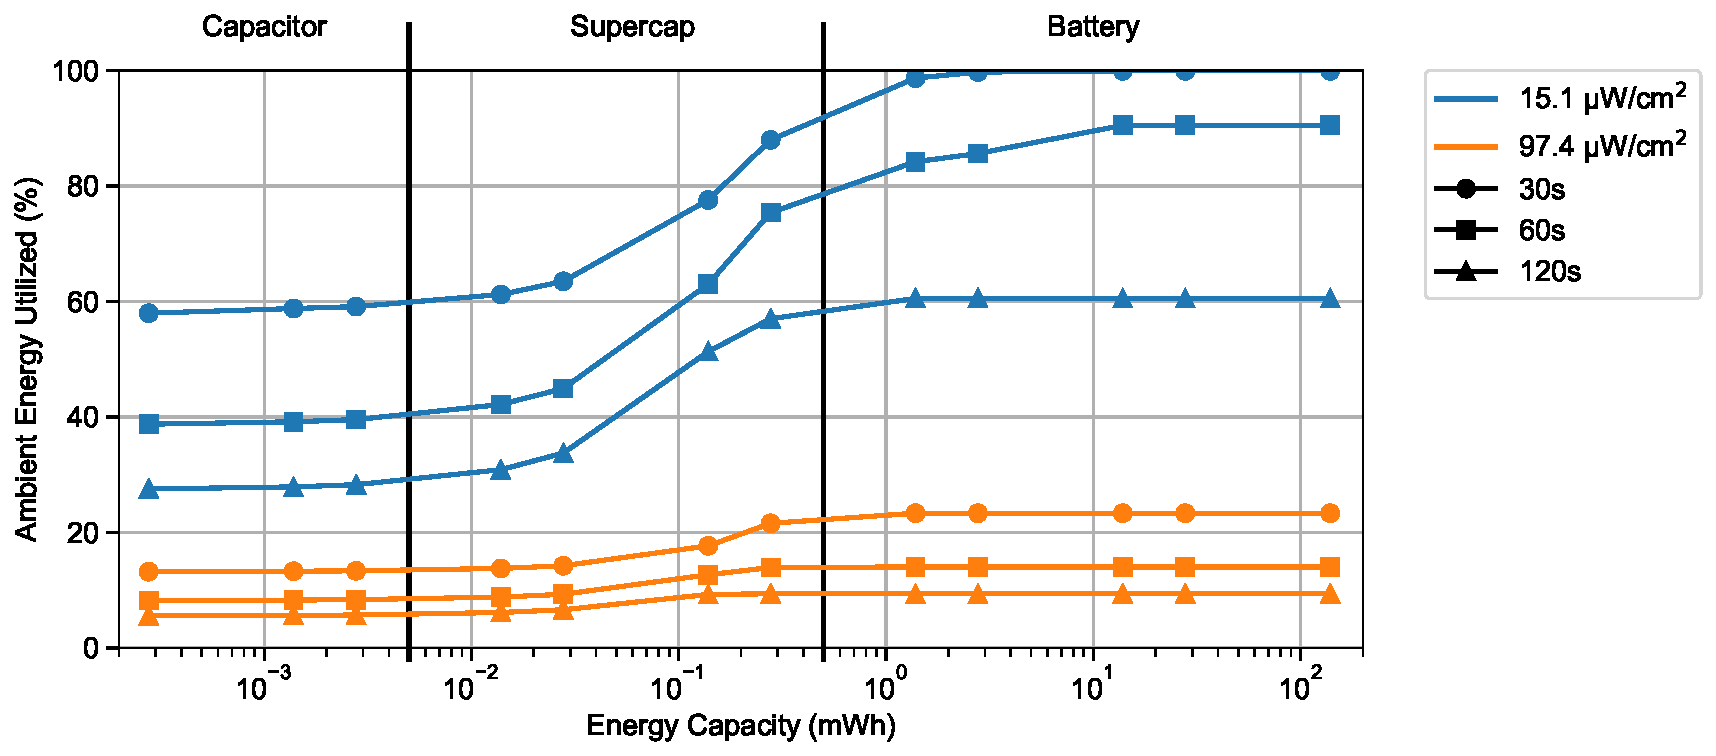
\includegraphics[width=\linewidth]{figs/capacity/sense_and_send/usage_reliability_v_secondary_capacity/usage_vs_secondary_size.pdf}
    \caption{Periodic application}
    \label{fig:usage:sensesec}
  \end{subfigure}
  \begin{subfigure}{\columnwidth}
    \centering
    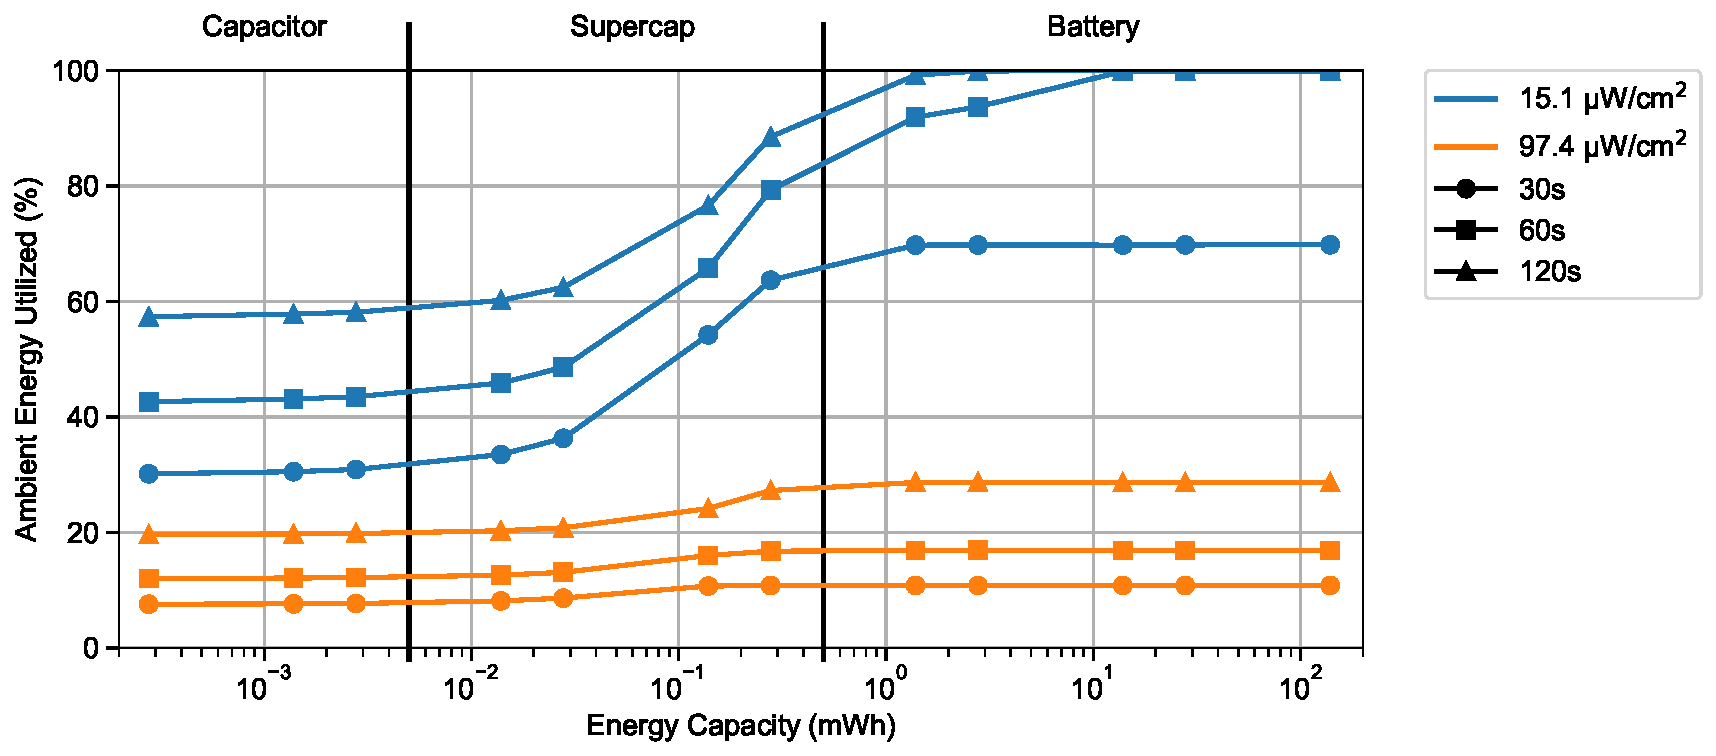
\includegraphics[width=\linewidth]{figs/capacity/door_occupancy/usage_vs_secondary_size}
    \caption{Reactive application}
    \label{fig:usage:eventsec}
  \end{subfigure}
  \caption{\normalfont Ambient energy utilization
    as a function of idealized secondary storage capacity for different
    harvesting scenarios and workloads. The harvesting scenarios and workloads
    are described in \cref{tab:capacity:rep}.
    \Cref{fig:usage:sensesec} represents the energy utilized by a periodic sense and send application, while \cref{fig:usage:eventsec} is the energy utilized by a event-driven application.
    Despite these two workloads exhibiting different event distributions and variance, the overall energy utilization follows the same trend with energy capacity. 
    As energy storage increases, the harvestable energy used in
    the application also increases. %implying
    %increased application performance.  
    Some scenarios, such as the periodic
    30\,s, 15.1\,\uW/cm\textsuperscript{2} case, reach 100\% utilization at
    sufficient secondary capacities indicating that all of the available energy is captured and may not
    be enough to meet the application's requirements.
    Generally, for both workloads and irradiance traces, from
    the smallest to largest capacity simulated, we see a 1.4-2.3x increase in
    utilized energy.
    }
\end{definefigure*}

\begin{definefigure*}{fig:capacity:availability}
  \centering
  \begin{subfigure}{\columnwidth}
    \centering
    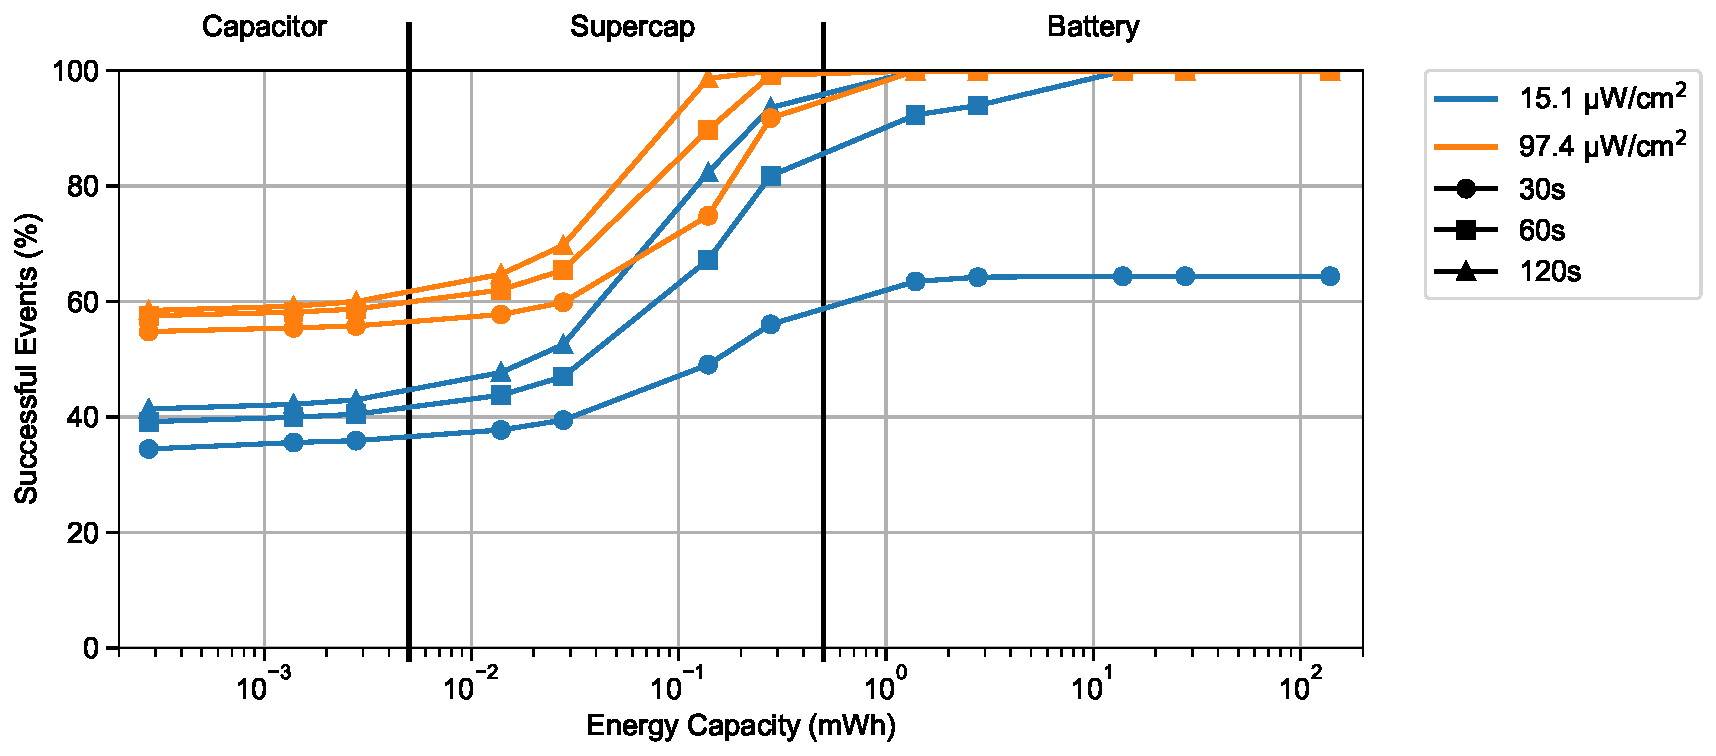
\includegraphics[width=\linewidth]{figs/capacity/sense_and_send/usage_reliability_v_secondary_capacity/events_vs_secondary_size.pdf}
      \caption{Periodic application}
    \label{fig:capacity:availability:sensesec}
  \end{subfigure}
  \begin{subfigure}{\columnwidth}
    \centering
    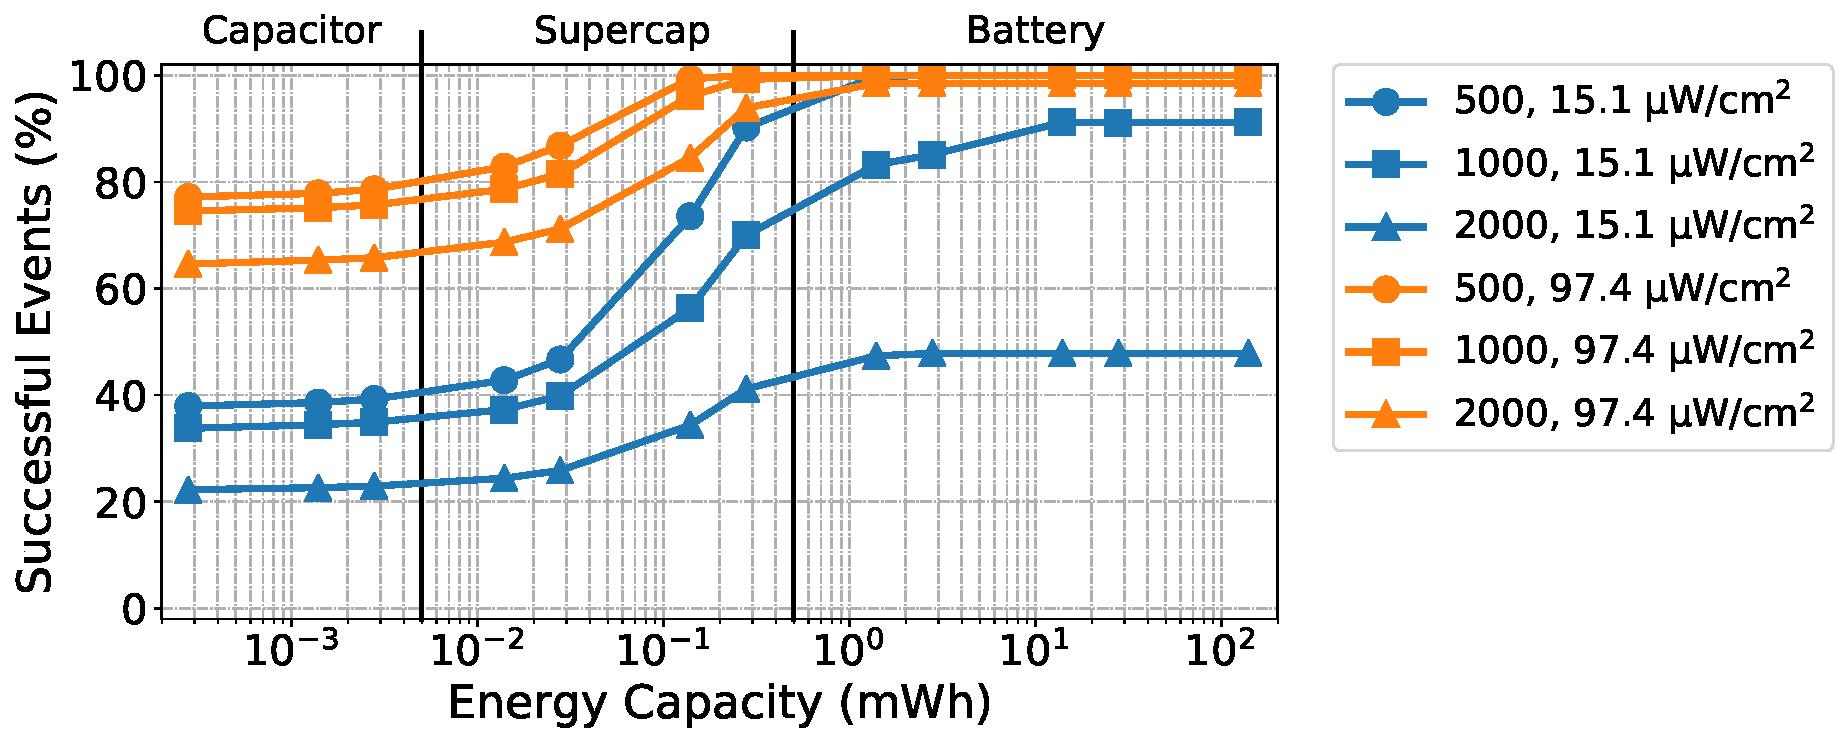
\includegraphics[width=\linewidth]{figs/capacity/door_occupancy/events_vs_secondary_size}
    \caption{Reactive application}
    \label{fig:capacity:availability:eventsec}
  \end{subfigure}
  \caption{
    \normalfont
    Workload availability
    for different harvesting scenarios, workloads, and idealized secondary storage sizes.
    We define availability as the percentage of successfully completed events. If a periodic or random event occurs and the sensor does not have sufficient energy to complete the event, that event is not completed and is considered missed.
    As expected, workload availability follows a similar 
    trend as energy utilization, improving with increased secondary energy
    storage and energy capture. 
    For both periodic and reactive workloads, from the smallest to
    largest capacity simulated, we see a 1.4-2.7x improvement in availability.
    In cases where average harvester power is sufficient to power the workload completely, the sensor achieves 100\% availability on the workload when configured with sufficient capacity.
    }
\end{definefigure*}

\begin{definefigure}{fig:capacity:period}
      \centering
      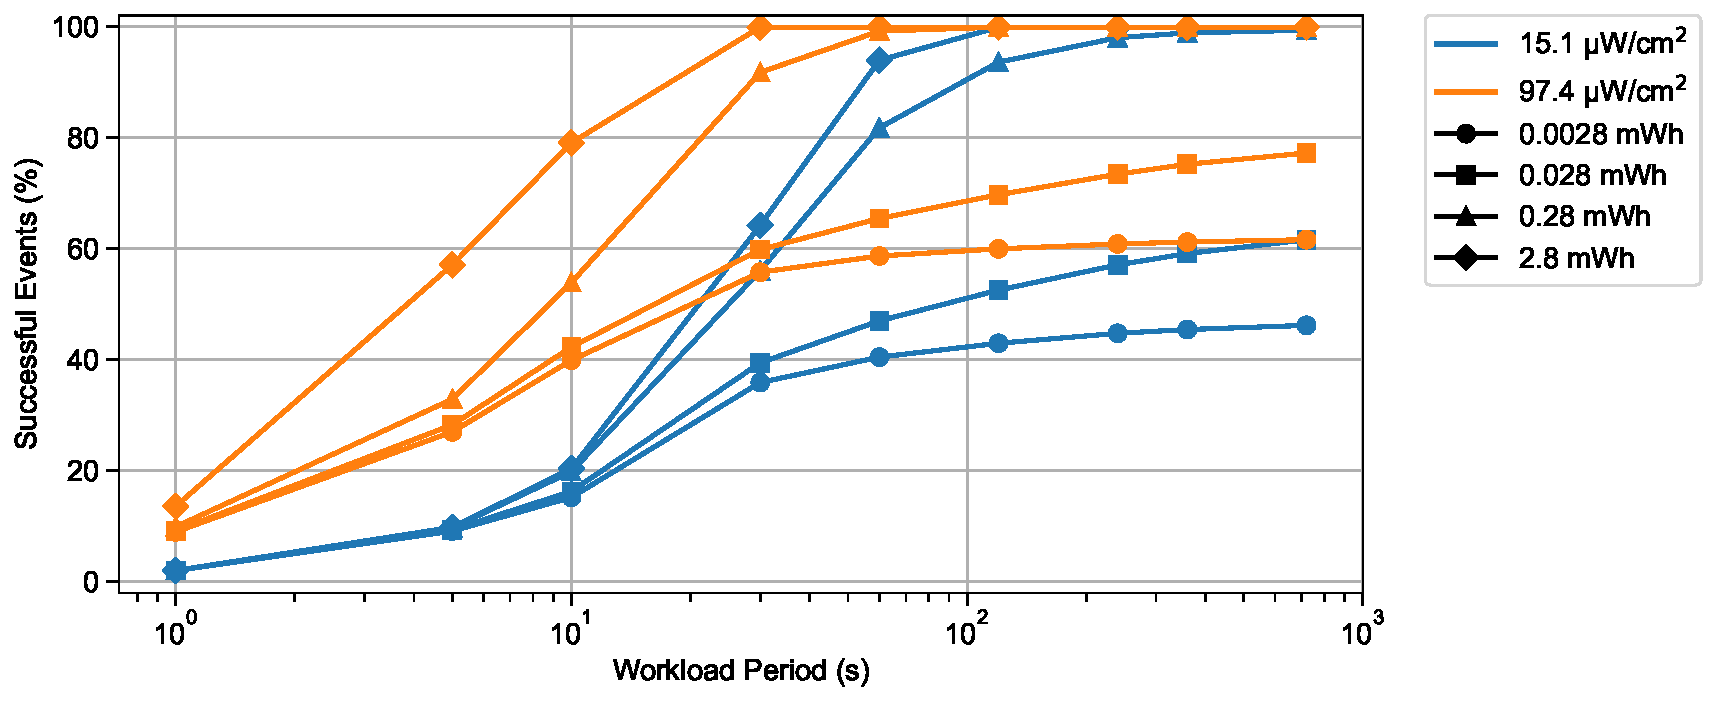
\includegraphics[width=\linewidth]{figs/capacity/sense_and_send/usage_reliability_v_period/events_vs_period.pdf}
    \caption{
    The performance of workloads with different periodicity with four decades of energy capacity.
    We investigate the period at which different secondary storage sizes
    meet a specific availability, showing that even with infrequent periodic
    workloads, small amounts of secondary storage have low availability while
    larger secondary stores approach 100\% availability. 
    } 
\end{definefigure}
    
\begin{definefigure}{fig:capacity:ttc}
      \centering
      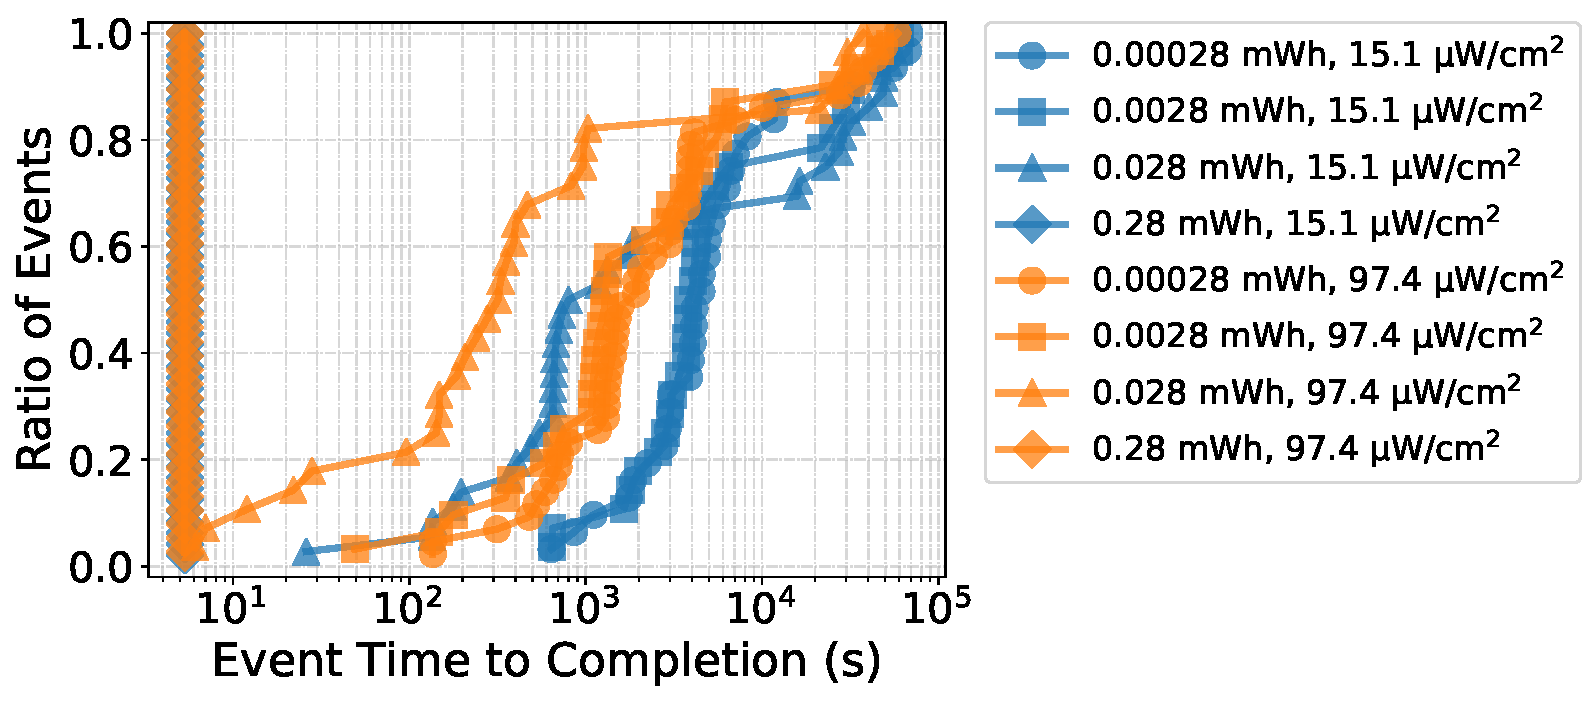
\includegraphics[width=\linewidth]{figs/capacity/ota_update/ttc_ota}
      \caption{
      A CDF of time to completion of a long-running, high energy event.
        In this
        workload, events are not atomic, and can be paused and resumed based on
        available energy. With secondary capacities that are large relative to the
        workload (which takes 93\,mJ) we see immediate completion.
        However, performing the event on smaller secondary capacities can take
        between three hours and a day to complete even for scenarios with large
        amounts of harvestable ambient energy.
      }
\end{definefigure}

\begin{definetable}{tab:capacity:rep}
    \begin{threeparttable}
    \centering
    \begin{subtable}{\columnwidth}
            \begin{tabularx}{\columnwidth}{@{\extracolsep{\fill}} l | c | c | c | c }
                Irradiance Trace  & Total Days & \thead{\\ Average Power\\(\textmu W/cm\textsuperscript{2})} & \thead{90\textsuperscript{th} Percentile\\Daily Power \\(\textmu W/cm\textsuperscript{2})} & \thead{10\textsuperscript{th} Percentile\\Daily Power \\(\textmu W/cm\textsuperscript{2})} \\\hline
                EnHANTs A   & 394  & 15.1     & 25.0      & 5.2\\
                EnHANTs D   & 311  & 97.4     & 256.5     & 24.8\\
                %Enhants C   & 327  & 745.4    & 1610.0    & 176.1\\
            \end{tabularx}
            \caption{Indoor photovoltaic irradiance traces}
            \label{tab:capacity:rep_trace}
        \end{subtable}\\
        \vspace{1em}
        \begin{subtable}{\columnwidth}
            \centering
            \begin{tabularx}{\columnwidth}{@{\extracolsep{\fill}} l | c | c | c }
                Workload Class & Energy per Event (uJ) & Average Period & Average Power (\textmu W)\,\tnote{a}\\\hline
            \multirow{4}{*}{Periodic}   & \multirow{4}{*}{586}  & 10\,s                 &  58.6     \\
                                        &                       & 30\,s                 &  24.5     \\
                                        &                       & 60\,s                 &  14.7     \\
                                        &                       & 120\,s                &  9.8      \\\hline
            \multirow{3}{*}{Reactive}   & \multirow{3}{*}{86}   & 3.4\,s\,\tnote{b}     &  25.3     \\
                                        &                       & 6.8\,s\,\tnote{b}     &  17.6     \\
                                        &                       & 13.6\,s\,\tnote{b}    &  11.3     \\\hline
                 Long-Running           & 93,300                 & 2\,weeks\,\tnote{c}  &  5.1      \\
            \end{tabularx}
            \caption{Representative workloads}
            \label{tab:capacity:rep_work}
        \end{subtable}
        \vspace{1em}
    \end{threeparttable}
    \small
    \begin{tablenotes}[para]
    \item[a] Average power includes an average 5\,\textmu W idle power, measured in \cref{sec:impl:permamote}.\\
    \item[b] Event times are based on a Poisson distribution for each hour of the day and drawn every second. The distribution is parameterized by collected entryway data then scaled.\\
    \item[c] Event time is based on a uniform distribution and drawn every second.
    \end{tablenotes}
    \caption{\normalfont Representative harvesting conditions and workloads.
    To evaluate different energy harvesting storage techniques, we define a set of energy harvesting
    conditions and workloads that are representative of common sensing applications. We choose two
    real irradiance traces with different magnitudes and distributions of available energy.
    These traces are summarized in \cref{tab:capacity:rep_trace}.
    We define three
    workloads: periodic, reactive, and long-running, and we characterize those workloads
    for different event frequencies. The energy used for each event is measured
    on our reference hardware described in \cref{sec:impl:permamote}.
    Statistics for the three workloads are described in \cref{tab:capacity:rep_work}.
    }
\end{definetable}

\begin{definetable}{tab:parameters}
    \centering
    \begin{tabularx}{\columnwidth}{@{\extracolsep{\fill}} lll}
\hline
\textbf{Config Type}& \multicolumn{1}{l}{\textbf{Parameter}}                   & \multicolumn{1}{l}{\textbf{Description}} \\ \hline
\textbf{Device}     & \texttt{operating\_voltage}                              & Output voltage of the power subsystem    \\
                    & \texttt{boost\_efficiency}                               & Efficiency of the boost converter        \\
                    & \texttt{frontend\_efficiency}                            & Efficiency of the harvesting frontend    \\ \hline
\textbf{Secondary}  & \texttt{capacity}                                        & Capacity of secondary in joules or mAh   \\
                    & \texttt{esr}                                             & Equivalent series resistance in ohms     \\
                    & \texttt{leakage\_constant}                               & Factor for capacity dependent leakage    \\
                    & \texttt{\string{max, min\string}\_hyst}                  & Secondary capacity upper/lower hysteresis\\ \hline
\textbf{Primary}    & \texttt{capacity}                                        & Capacity of primary in mAh               \\
                    & \texttt{leakage\_percent}                                & Percent capacity leakage per year        \\ \hline
        \textbf{Harvester}  & \texttt{area}                                    & Area of solar harvester in cm\textsuperscript{2}\\
\textbf{(Solar)}    & \texttt{efficiency}                                      & Efficiency of solar panel                \\ \hline
%\textbf{Workload}   & \texttt{type}                                            & Periodic or Reactive                     \\
%                    & \texttt{period/scale}                                    & Period, or scale for average \# of events \\
%                    & \texttt{opportunistic}                                   & Ignore period, and perform events ASAP   \\
%                    & \texttt{sleep\_current}                                  & Current draw of system in low power mode \\
%                    & \texttt{startup\_\string{energy, period\string}}         & Energy, time required for startup        \\
%                    & \texttt{event\_\string{energy, period\string}}           & Total energy, time required for work event \\
%                    & \texttt{atomic}                                          & Workload is atomic, or intermittent      \\
%                    & \texttt{event\_period\_min}                              & If not atomic, minimum splitable period  \\ \hline

    \end{tabularx}
    \caption{\normalfont Simulation configuration parameters.
      A subset of available configuration options for the sensor energy simulation. 
      Simulated sensors can be configured to use 
      secondary storage and an energy harvester, a
      primary-cell, or both. A secondary-cell can be configured with a
      hysteresis, with a lower bound set to \texttt{min\_hyst}
      and an upper bound of \texttt{max\_hyst}.
      %This upper bound must represent
      %the minimum amount of
      %energy to do useful work.
      %Therefore, the upper bound of charging
      %hysteresis is set to \texttt{secondary\_max\_hyst}.
      %Workloads are
      %configured to be either periodic or reactive, and workload intensity is
      %determined by period, or a scaling factor determining the average number
      %of events picked from a random distribution.
      }
\end{definetable}
\begin{definefigure}{fig:capacity:statemachine}
    \centering
    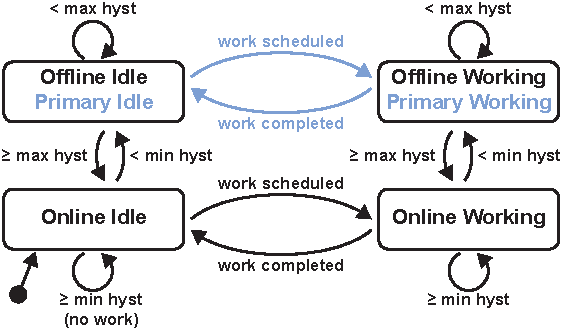
\includegraphics[width=\columnwidth]{figs/capacity/model_state_machine}
    \caption{\normalfont Model state machine.
    A modeled device can be in one of four states: \textsf{Offline Idle},
    \textsf{Online Idle}, \textsf{Online Working}, and \textsf{Offline
    Working}. When a device is \textsf{Offline Idle}, it has run out of energy
    and is off. If a device is \textsf{Online
    Idle}, it is on and in deep sleep, ready to perform work if triggered. If
    triggered, a device moves to \textsf{Online Working}, where it performs a
    portion of a work event.  If a workload is atomic, workload events
    \textit{must} be completed in one \textsf{Online Working} step, without any
    transitions to an offline state.  \textsf{Offline Working} means that while
    working on a non-atomic task, the device ran out of energy, checkpointed,
    and is waiting to harvest more and resume its task.  For devices
    configured with a primary-cell, \textsf{Offline Idle} and \textsf{Offline
    Working} become \textsf{\textcolor{primary-blue}{Primary Idle}} and
    \textsf{\textcolor{primary-blue}{Primary Working}} respectively.  In these
    states, outgoing energy is charged against the primary-cell and the device
    remains online and able to perform work for the life of the primary-cell.
    %State transitions are determined by incoming energy, the state of charge of
    %the secondary storage, and the generated work schedule from workload
    %parameters.
    }
\end{definefigure}

\begin{definetable}{tab:capacity:components}
    \begin{threeparttable}
    \centering
        \begin{tabularx}{\columnwidth}{@{\extracolsep{\fill}} l | l | c | c}
            Component                           &  Function                     & Active Power          & Idle Power \\\hline
            \multirow{2}{*}{Nordic NRF52840}    & Processor                     & 56\,\uA/MHz           & 940\,nA\,\tnote{a}  \\
                                                & Radio                         & 5.2\,mA @ 0\,dbm      & \textemdash\,\tnote{a}\\
            Ambiq AB1815-T3                     & Real time clock               & 55\,nA                & N/A\,\tnote{b}  \\
            ST Micro LIS2DW12                   & Accelerometer                 & 1\,uA @ 12.5\,Hz      & 50\,nA  \\
            Maxim MAX44009                      & Light sensor                  & 650\,nA               & N/A\,\tnote{b}  \\
            Intersil ISL29125                   & Color sensor                  & 56\,\uA               & 500\,nA  \\
            Silicon Labs SI7021                 & Humidty sensor& 1.5\,\uA @ 1\,Hz      & 60\,nA  \\
            TE Connectivity MS5637              & Pressure sensor               & 0.6 - 5\,\uA @ 1\,Hz  & 10\,nA  \\
            Panasonic EKMB11011                 & PIR Occupancy                 & 100\,\uA              & 1\,uA  \\
        \end{tabularx}
    \end{threeparttable}
    \begin{tablenotes}[para]
    \item[a] Sleep current for both processor and radio.
    \item[b] No shutdown or idle mode.
    \end{tablenotes}
    \caption{
    The components used by our representative hardware. Benchmarks of the processor, radio, and sensors presented here are used to establish our representative workloads used by our wireless sensor energy simulation.
    These components are among the lowest power options available, and
    are even 2-4x lower power than those used on relatively recent
    systems~\cite{hesterFlicker17,andersen2017hamilton,colinReconfigurable18}. 
    }
    %Technology
    %scaling for embedded sensors, processors, and radios
    %has driven down the average power of a sensor node much closer to the
    %harvestable solar energy available in indoor lighting conditions. This allows
    %more systems to subsist or achieve extended lifetimes through energy harvesting.
\end{definetable}

